\documentclass[border=2pt]{standalone}
\usepackage{amsmath, amsthm, amsfonts}
\usepackage{tikz-cd, kotex}
\usepackage{ytableau}
\usepackage{quiver}
\usepackage{Operators}
\usepackage{palette}
\usepackage{diagram-style}
\usetikzlibrary{arrows.meta, positioning, decorations.pathreplacing, decorations.markings, intersections}
\begin{document}

%%FIG diagram (Postnikov_Diagram_and_Plabic_Graph-1.svg)
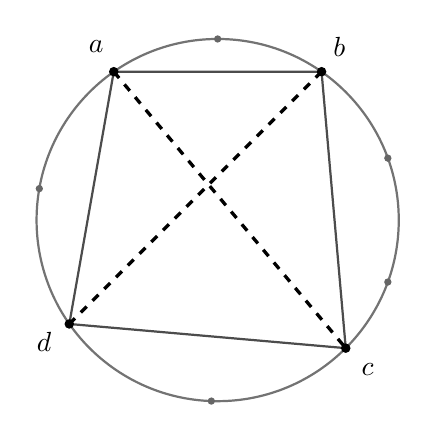
\begin{tikzpicture}[scale=1.15]
  \def\R{2}
  \draw[black!55, thick] (0,0) circle (\R);
  \coordinate (a) at (125:\R);
  \coordinate (b) at (55:\R);
  \coordinate (c) at (315:\R);
  \coordinate (d) at (215:\R);
  \draw[black!70, thick] (a)--(b)--(c)--(d)--cycle;        % 변 (비교차 현)
  \draw[black, very thick, dashed] (a)--(c);               % 대각선 (교차 현)
  \draw[black, very thick, dashed] (b)--(d);
  \foreach \ang in {90, 20, 340, 268, 170}{                % S에 해당하는 회색 점
    \fill[black!60] (\ang:\R) circle (1.15pt);
  }
  \fill[black] (a) circle (1.5pt);
  \fill[black] (b) circle (1.5pt);
  \fill[black] (c) circle (1.5pt);
  \fill[black] (d) circle (1.5pt);
  \node at (125:{\R+0.34}) {$a$};
  \node at (55:{\R+0.34})  {$b$};
  \node at (315:{\R+0.34}) {$c$};
  \node at (215:{\R+0.34}) {$d$};
\end{tikzpicture}

%%FIG diagram (Postnikov_Diagram_and_Plabic_Graph-2.svg)
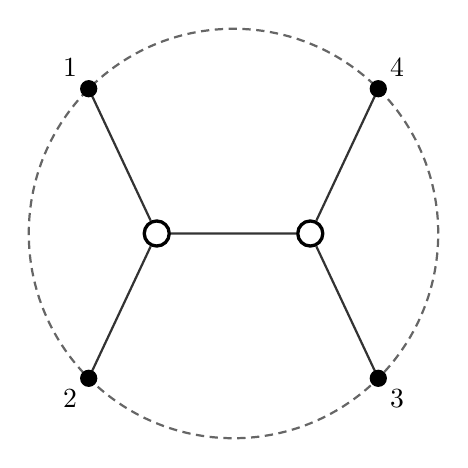
\begin{tikzpicture}[scale=1.3, >=Stealth,
   wv/.style={draw=black, very thick, fill=none, circle, inner sep=3.2pt}]
  \def\R{2}
  \draw[black!60, thick, densely dashed] (0,0) circle (\R);
  \node[wv] (W1) at (-0.75,0) {};
  \node[wv] (W2) at (0.75,0) {};
  \coordinate (b1) at (135:\R); \coordinate (b2) at (225:\R);
  \coordinate (b3) at (315:\R); \coordinate (b4) at (45:\R);
  \draw[black!80, thick] (W1)--(b1) (W1)--(b2) (W1)--(W2) (W2)--(b3) (W2)--(b4);
  \foreach \p/\lab/\pos in {b1/1/{above left}, b2/2/{below left}, b3/3/{below right}, b4/4/{above right}}{
     \fill[black] (\p) circle (2.4pt); \node[\pos=1pt] at (\p) {$\lab$}; }
\end{tikzpicture}

%%FIG diagram (Postnikov_Diagram_and_Plabic_Graph-3.svg)
\begin{tikzpicture}[scale=1.3, >=Stealth,
   wv/.style={draw=black, very thick, fill=none, circle, inner sep=3.2pt},
   trip/.style={accent1, line width=1.9pt, postaction={decorate,
      decoration={markings, mark=at position #1 with {\arrow{Stealth[length=3.2mm]}}}}}]
  \def\R{2}
  \draw[black!60, thick, densely dashed] (0,0) circle (\R);
  \node[wv] (W1) at (-0.75,0) {}; \node[wv] (W2) at (0.75,0) {};
  \coordinate (b1) at (135:\R); \coordinate (b2) at (225:\R);
  \coordinate (b3) at (315:\R); \coordinate (b4) at (45:\R);
  \draw[black!80, thick] (W1)--(b1) (W2)--(b4);
  \draw[trip=0.52] (b2)--(W1)--(W2)--(b3);
  \foreach \p/\lab/\pos in {b1/1/{above left}, b2/2/{below left}, b3/3/{below right}, b4/4/{above right}}{
     \fill[black] (\p) circle (2.4pt); \node[\pos=1pt] at (\p) {$\lab$}; }
\end{tikzpicture}

%%FIG diagram (Postnikov_Diagram_and_Plabic_Graph-4.svg)
\begin{tikzpicture}[scale=1.3, >=Stealth,
   wv/.style={draw=black, very thick, fill=none, circle, inner sep=3.2pt},
   trip/.style={accent1, line width=1.9pt, postaction={decorate,
      decoration={markings, mark=at position #1 with {\arrow{Stealth[length=3.2mm]}}}}}]
  \def\R{2}
  \draw[black!60, thick, densely dashed] (0,0) circle (\R);
  \node[wv] (W) at (0,0) {};
  \coordinate (b1) at (135:\R); \coordinate (b2) at (225:\R);
  \coordinate (b3) at (315:\R); \coordinate (b4) at (45:\R);
  \draw[black!80, thick] (W)--(b1) (W)--(b4);
  \draw[trip=0.6] (b2)--(W)--(b3);
  \foreach \p/\lab/\pos in {b1/1/{above left}, b2/2/{below left}, b3/3/{below right}, b4/4/{above right}}{
     \fill[black] (\p) circle (2.4pt); \node[\pos=1pt] at (\p) {$\lab$}; }
\end{tikzpicture}

%%FIG diagram (Postnikov_Diagram_and_Plabic_Graph-5.svg)
\begin{tikzpicture}[scale=1.3, >=Stealth,
   strand/.style={line width=1.5pt, postaction={decorate,
      decoration={markings, mark=at position 0.5 with {\arrow{Stealth[length=3mm]}}}}},
   bare/.style={line width=1.5pt}]
  \def\R{2}
  \draw[black!55, thick, densely dashed] (0,0) circle (\R);
  \coordinate (b1) at (90:\R); \coordinate (b2) at (180:\R);
  \coordinate (b3) at (270:\R); \coordinate (b4) at (0:\R);
  \draw[strand, accent1!75!black,    name path=sR] (b1) .. controls (-1.35,0.85) and (-1.35,-0.85) .. (b3);
  \draw[strand, accent2!70!black,   name path=sB] (b2) .. controls (-0.85,1.35) and (0.85,1.35) .. (b4);
  \draw[strand, accent3!55!black,  name path=sG] (b3) .. controls (1.35,-0.85) and (1.35,0.85) .. (b1);
  \draw[strand, accent1!90!black, name path=sO] (b4) .. controls (0.85,-1.35) and (-0.85,-1.35) .. (b2);
  \path[name intersections={of=sR and sB, name=cNW}];
  \path[name intersections={of=sB and sG, name=cNE}];
  \path[name intersections={of=sG and sO, name=cSE}];
  \path[name intersections={of=sO and sR, name=cSW}];
  \fill[white] (cNW-1) circle (4pt);
  \begin{scope}\clip (cNW-1) circle (5.5pt);\draw[bare, accent1!75!black] (b1) .. controls (-1.35,0.85) and (-1.35,-0.85) .. (b3);\end{scope}
  \fill[white] (cNE-1) circle (4pt);
  \begin{scope}\clip (cNE-1) circle (5.5pt);\draw[bare, accent2!70!black] (b2) .. controls (-0.85,1.35) and (0.85,1.35) .. (b4);\end{scope}
  \fill[white] (cSE-1) circle (4pt);
  \begin{scope}\clip (cSE-1) circle (5.5pt);\draw[bare, accent3!55!black] (b3) .. controls (1.35,-0.85) and (1.35,0.85) .. (b1);\end{scope}
  \fill[white] (cSW-1) circle (4pt);
  \begin{scope}\clip (cSW-1) circle (5.5pt);\draw[bare, accent1!90!black] (b4) .. controls (0.85,-1.35) and (-0.85,-1.35) .. (b2);\end{scope}
  \foreach \p/\lab/\pos in {b1/1/{above}, b2/2/{left}, b3/3/{below}, b4/4/{right}}{
     \fill[black] (\p) circle (1.7pt); \node[\pos=2pt] at (\p) {$\lab$}; }
\end{tikzpicture}

%%FIG diagram (Postnikov_Diagram_and_Plabic_Graph-6.svg)
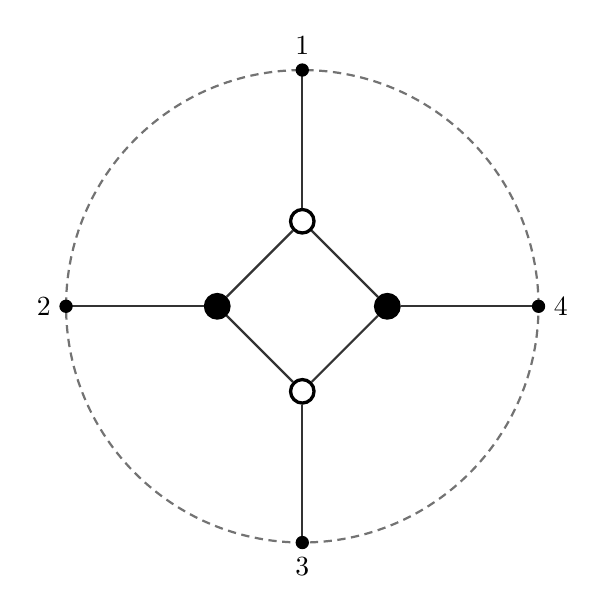
\begin{tikzpicture}[scale=1.5, >=Stealth,
   bdot/.style={fill=black, circle, inner sep=1.7pt},
   wv/.style={draw=black, very thick, fill=none, circle, inner sep=3pt},
   bv/.style={draw=black, very thick, fill=black, circle, inner sep=3pt}]
  \def\R{2}
  \draw[black!55, thick, densely dashed] (0,0) circle (\R);
  \node[wv] (N) at (0,0.72) {}; \node[bv] (E) at (0.72,0) {};
  \node[wv] (S) at (0,-0.72) {}; \node[bv] (W) at (-0.72,0) {};
  \coordinate (b1) at (90:\R); \coordinate (b2) at (180:\R);
  \coordinate (b3) at (270:\R); \coordinate (b4) at (0:\R);
  \draw[black!80, thick] (N)--(E)--(S)--(W)--(N);
  \draw[black!80, thick] (N)--(b1) (W)--(b2) (S)--(b3) (E)--(b4);
  \foreach \p/\lab/\pos in {b1/1/{above}, b2/2/{left}, b3/3/{below}, b4/4/{right}}{
     \node[bdot] at (\p) {}; \node[\pos=2pt] at (\p) {$\lab$}; }
\end{tikzpicture}

%%FIG diagram (Postnikov_Diagram_and_Plabic_Graph-7.svg)
\begin{tikzpicture}[scale=1.0, >=Stealth,
   str/.style={line width=1.4pt, postaction={decorate,
      decoration={markings, mark=at position #1 with {\arrow{Stealth[length=2.6mm]}}}}}, str/.default=0.58]
  %% left: moving strand bulges left, triangle PQR sits on the left (Q,R on the two black strands)
  \begin{scope}[shift={(-2.6,0)}]
    \fill[accent1!10] (0,0) -- (-0.5,-0.7)
        .. controls (-0.72,-0.25) and (-0.72,0.25) .. (-0.5,0.7) -- cycle;   % 정직한 삼각형, 한 변=빨간 strand arc
    \draw[str=0.70, black] (-1,-1.4) -- (1,1.4);                                 % 멈춰있는 strand
    \draw[str=0.70, black] (1,-1.4) -- (-1,1.4);                                 % 멈춰있는 strand
    \draw[str, accent1]   (0,-1.4) -- (-0.5,-0.7)                               % 움직이는 strand (위, 빨강)
        .. controls (-0.72,-0.25) and (-0.72,0.25) .. (-0.5,0.7) -- (0,1.4);
  \end{scope}
  \node at (0,0) {$\longleftrightarrow$};
  %% right: moving strand bulges right (mirror image)
  \begin{scope}[shift={(2.6,0)}]
    \fill[accent1!10] (0,0) -- (0.5,-0.7)
        .. controls (0.72,-0.25) and (0.72,0.25) .. (0.5,0.7) -- cycle;
    \draw[str=0.70, black] (1,-1.4) -- (-1,1.4);
    \draw[str=0.70, black] (-1,-1.4) -- (1,1.4);
    \draw[str, accent1]   (0,-1.4) -- (0.5,-0.7)
        .. controls (0.72,-0.25) and (0.72,0.25) .. (0.5,0.7) -- (0,1.4);
  \end{scope}
\end{tikzpicture}

%%FIG diagram (Postnikov_Diagram_and_Plabic_Graph-8.svg)
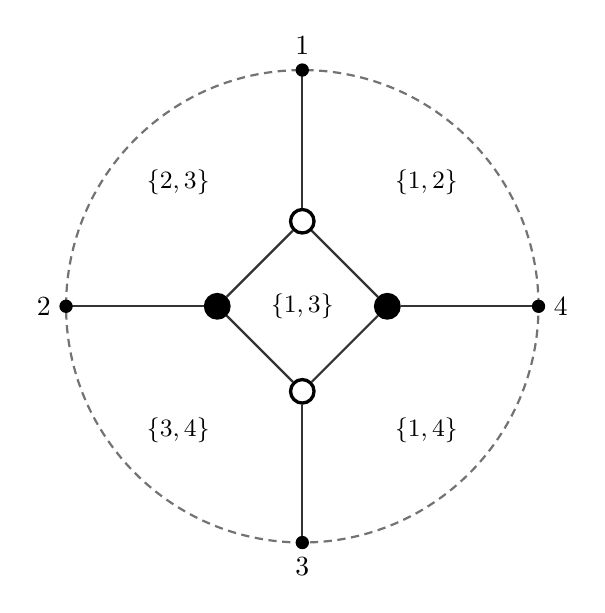
\begin{tikzpicture}[scale=1.5, >=Stealth,
   bdot/.style={fill=black, circle, inner sep=1.7pt},
   wv/.style={draw=black, very thick, fill=none, circle, inner sep=3pt},
   bv/.style={draw=black, very thick, fill=black, circle, inner sep=3pt}]
  \def\R{2}
  \draw[black!55, thick, densely dashed] (0,0) circle (\R);
  \node[wv] (N) at (0,0.72) {}; \node[bv] (E) at (0.72,0) {};
  \node[wv] (S) at (0,-0.72) {}; \node[bv] (W) at (-0.72,0) {};
  \coordinate (b1) at (90:\R); \coordinate (b2) at (180:\R);
  \coordinate (b3) at (270:\R); \coordinate (b4) at (0:\R);
  \draw[black!80, thick] (N)--(E)--(S)--(W)--(N);
  \draw[black!80, thick] (N)--(b1) (W)--(b2) (S)--(b3) (E)--(b4);
  \foreach \p/\lab/\pos in {b1/1/{above}, b2/2/{left}, b3/3/{below}, b4/4/{right}}{
     \node[bdot] at (\p) {}; \node[\pos=2pt] at (\p) {$\lab$}; }
  \node[font=\small] at (0,0) {$\{1,3\}$};
  \node[font=\small] at (1.05,1.05) {$\{1,2\}$};
  \node[font=\small] at (-1.05,1.05) {$\{2,3\}$};
  \node[font=\small] at (-1.05,-1.05) {$\{3,4\}$};
  \node[font=\small] at (1.05,-1.05) {$\{1,4\}$};
\end{tikzpicture}

%%FIG diagram (Postnikov_Diagram_and_Plabic_Graph-9.svg)
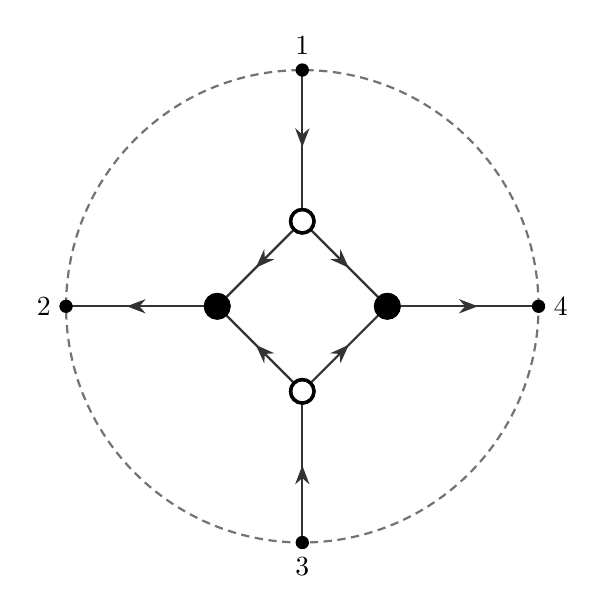
\begin{tikzpicture}[scale=1.5, >=Stealth,
   bdot/.style={fill=black, circle, inner sep=1.7pt},
   wv/.style={draw=black, very thick, fill=none, circle, inner sep=3pt},
   bv/.style={draw=black, very thick, fill=black, circle, inner sep=3pt},
   dedge/.style={black!80, thick, postaction={decorate,
      decoration={markings, mark=at position 0.56 with {\arrow{Stealth[length=2.4mm]}}}}}]
  \def\R{2}
  \draw[black!55, thick, densely dashed] (0,0) circle (\R);
  \node[wv] (N) at (0,0.72) {}; \node[bv] (E) at (0.72,0) {};
  \node[wv] (S) at (0,-0.72) {}; \node[bv] (W) at (-0.72,0) {};
  \coordinate (b1) at (90:\R); \coordinate (b2) at (180:\R);
  \coordinate (b3) at (270:\R); \coordinate (b4) at (0:\R);
  \draw[dedge] (N)--(E); \draw[dedge] (N)--(W);
  \draw[dedge] (S)--(E); \draw[dedge] (S)--(W);
  \draw[dedge] (b1)--(N); \draw[dedge] (b3)--(S);
  \draw[dedge] (E)--(b4); \draw[dedge] (W)--(b2);
  \node[wv] at (N) {}; \node[bv] at (E) {}; \node[wv] at (S) {}; \node[bv] at (W) {};
  \foreach \p/\lab/\pos in {b1/1/{above}, b2/2/{left}, b3/3/{below}, b4/4/{right}}{
     \node[bdot] at (\p) {}; \node[\pos=2pt] at (\p) {$\lab$}; }
\end{tikzpicture}

%%FIG diagram (Postnikov_Diagram_and_Plabic_Graph-10.svg)
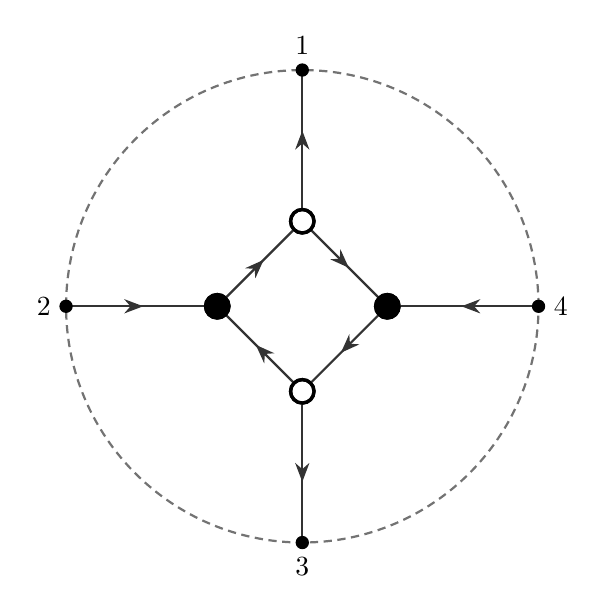
\begin{tikzpicture}[scale=1.5, >=Stealth,
   bdot/.style={fill=black, circle, inner sep=1.7pt},
   wv/.style={draw=black, very thick, fill=none, circle, inner sep=3pt},
   bv/.style={draw=black, very thick, fill=black, circle, inner sep=3pt},
   dedge/.style={black!80, thick, postaction={decorate,
      decoration={markings, mark=at position 0.56 with {\arrow{Stealth[length=2.4mm]}}}}}]
  \def\R{2}
  \draw[black!55, thick, densely dashed] (0,0) circle (\R);
  \node[wv] (N) at (0,0.72) {}; \node[bv] (E) at (0.72,0) {};
  \node[wv] (S) at (0,-0.72) {}; \node[bv] (W) at (-0.72,0) {};
  \coordinate (b1) at (90:\R); \coordinate (b2) at (180:\R);
  \coordinate (b3) at (270:\R); \coordinate (b4) at (0:\R);
  \draw[dedge] (W)--(N); \draw[dedge] (N)--(E);
  \draw[dedge] (E)--(S); \draw[dedge] (S)--(W);
  \draw[dedge] (b2)--(W); \draw[dedge] (b4)--(E);
  \draw[dedge] (N)--(b1); \draw[dedge] (S)--(b3);
  \node[wv] at (N) {}; \node[bv] at (E) {}; \node[wv] at (S) {}; \node[bv] at (W) {};
  \foreach \p/\lab/\pos in {b1/1/{above}, b2/2/{left}, b3/3/{below}, b4/4/{right}}{
     \node[bdot] at (\p) {}; \node[\pos=2pt] at (\p) {$\lab$}; }
\end{tikzpicture}

%%FIG diagram (Postnikov_Diagram_and_Plabic_Graph-11.svg)
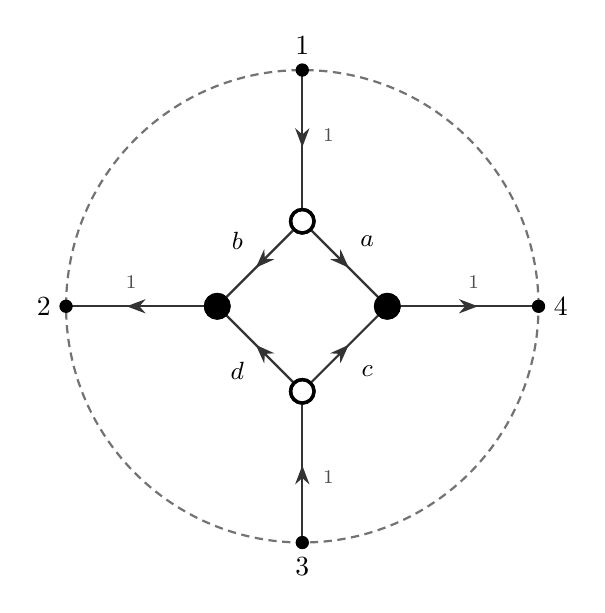
\begin{tikzpicture}[scale=1.5, >=Stealth,
   bdot/.style={fill=black, circle, inner sep=1.7pt},
   wv/.style={draw=black, very thick, fill=none, circle, inner sep=3pt},
   bv/.style={draw=black, very thick, fill=black, circle, inner sep=3pt},
   dedge/.style={black!80, thick, postaction={decorate,
      decoration={markings, mark=at position 0.56 with {\arrow{Stealth[length=2.4mm]}}}}}]
  \def\R{2}
  \draw[black!55, thick, densely dashed] (0,0) circle (\R);
  \node[wv] (N) at (0,0.72) {}; \node[bv] (E) at (0.72,0) {};
  \node[wv] (S) at (0,-0.72) {}; \node[bv] (W) at (-0.72,0) {};
  \coordinate (b1) at (90:\R); \coordinate (b2) at (180:\R);
  \coordinate (b3) at (270:\R); \coordinate (b4) at (0:\R);
  \draw[dedge] (N)--(E); \draw[dedge] (N)--(W);
  \draw[dedge] (S)--(E); \draw[dedge] (S)--(W);
  \draw[dedge] (b1)--(N); \draw[dedge] (b3)--(S);
  \draw[dedge] (E)--(b4); \draw[dedge] (W)--(b2);
  \node[wv] at (N) {}; \node[bv] at (E) {}; \node[wv] at (S) {}; \node[bv] at (W) {};
  \node[font=\small] at (0.55,0.55) {$a$};
  \node[font=\small] at (-0.55,0.55) {$b$};
  \node[font=\small] at (0.55,-0.55) {$c$};
  \node[font=\small] at (-0.55,-0.55) {$d$};
  \node[black!70, font=\scriptsize] at (0.22,1.45) {$1$};
  \node[black!70, font=\scriptsize] at (0.22,-1.45) {$1$};
  \node[black!70, font=\scriptsize] at (1.45,0.2) {$1$};
  \node[black!70, font=\scriptsize] at (-1.45,0.2) {$1$};
  \foreach \p/\lab/\pos in {b1/1/{above}, b2/2/{left}, b3/3/{below}, b4/4/{right}}{
     \node[bdot] at (\p) {}; \node[\pos=2pt] at (\p) {$\lab$}; }
\end{tikzpicture}

%%FIG diagram (Postnikov_Diagram_and_Plabic_Graph-12.svg)
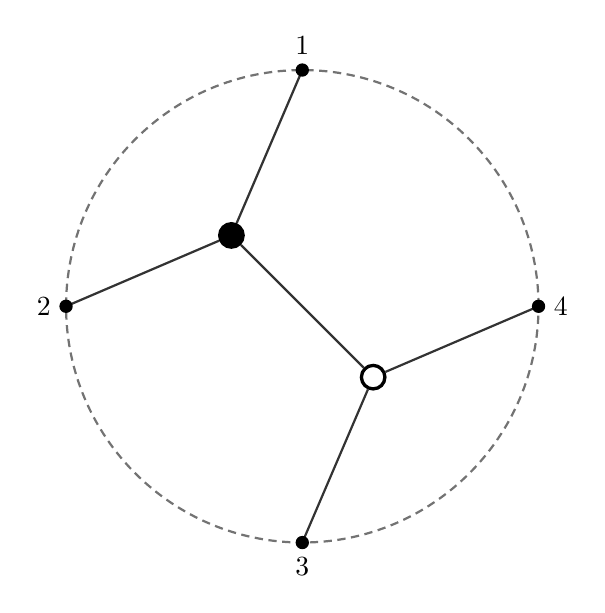
\begin{tikzpicture}[scale=1.5, >=Stealth,
   bdot/.style={fill=black, circle, inner sep=1.7pt},
   wv/.style={draw=black, very thick, fill=none, circle, inner sep=3pt},
   bv/.style={draw=black, very thick, fill=black, circle, inner sep=3pt}]
  \def\R{2}
  \draw[black!55, thick, densely dashed] (0,0) circle (\R);
  \node[bv] (W) at (-0.6,0.6) {};
  \node[wv] (S) at (0.6,-0.6) {};
  \coordinate (b1) at (90:\R); \coordinate (b2) at (180:\R);
  \coordinate (b3) at (270:\R); \coordinate (b4) at (0:\R);
  \draw[black!80, thick] (W)--(S);
  \draw[black!80, thick] (W)--(b1) (W)--(b2) (S)--(b3) (S)--(b4);
  \foreach \p/\lab/\pos in {b1/1/{above}, b2/2/{left}, b3/3/{below}, b4/4/{right}}{
     \node[bdot] at (\p) {}; \node[\pos=2pt] at (\p) {$\lab$}; }
\end{tikzpicture}

%%FIG diagram (Postnikov_Diagram_and_Plabic_Graph-13.svg)
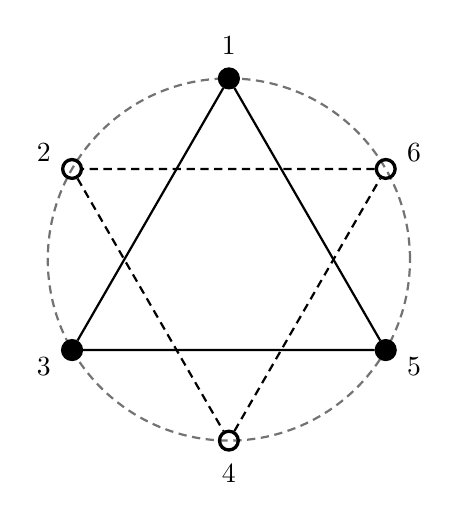
\begin{tikzpicture}[scale=1.15,
   bv/.style={draw=black, very thick, fill=black, circle, inner sep=2.4pt},
   wv/.style={draw=black, very thick, fill=none, circle, inner sep=2.4pt}]
  \def\R{2}
  \draw[black!55, thick, densely dashed] (0,0) circle (\R);
  \node[bv] (p1) at (90:\R) {};  \node[wv] (p2) at (150:\R) {};
  \node[bv] (p3) at (210:\R) {}; \node[wv] (p4) at (270:\R) {};
  \node[bv] (p5) at (330:\R) {}; \node[wv] (p6) at (30:\R) {};
  \draw[black, thick] (p1)--(p3) (p3)--(p5) (p5)--(p1);
  \draw[black, thick, densely dashed] (p2)--(p4) (p4)--(p6) (p6)--(p2);
  \foreach \ang/\lab in {90/1, 150/2, 210/3, 270/4, 330/5, 30/6}{
    \node at (\ang:{\R+0.36}) {$\lab$};
  }
\end{tikzpicture}

%%FIG diagram (Postnikov_Diagram_and_Plabic_Graph-14.svg)
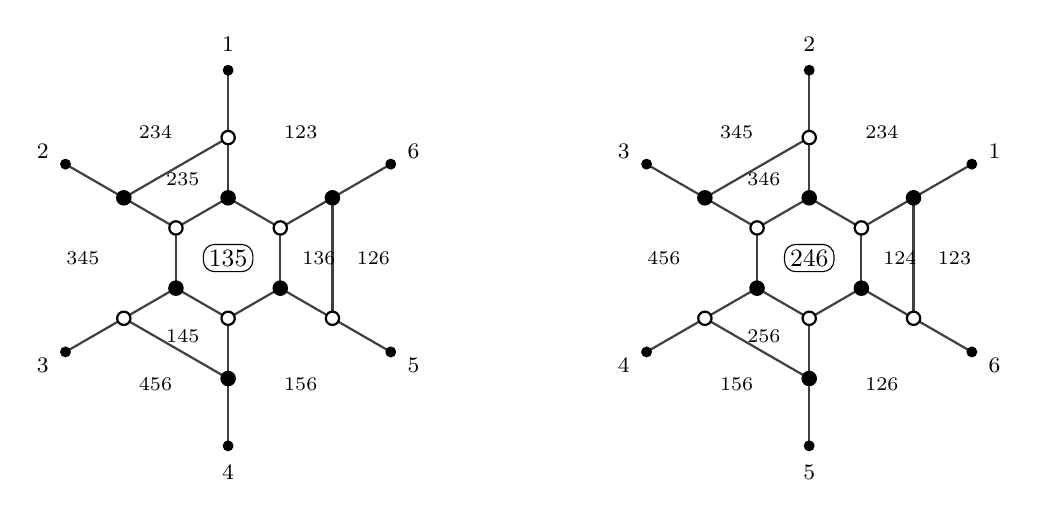
\begin{tikzpicture}[scale=0.9, >=Stealth,
   wv/.style={draw=black, thick, fill=white, circle, inner sep=1.7pt},
   bv/.style={draw=black, thick, fill=black, circle, inner sep=1.7pt},
   bdot/.style={fill=black, circle, inner sep=1.4pt},
   ge/.style={black!75, thick},
   fl/.style={font=\scriptsize},
   fc/.style={draw=black, rounded corners, inner sep=2pt, font=\small}]
  % ---------- LEFT: {135}-seed ----------
  \begin{scope}[shift={(-4.1,0)}]
    \foreach \nm/\ang/\rad in {W1/30/0.85,B3/90/0.85,W3/150/0.85,B2/210/0.85,W2/270/0.85,B1/330/0.85,W4/90/1.7,B4/150/1.7,W5/210/1.7,B5/270/1.7,W6/330/1.7,B6/30/1.7}{ \coordinate (\nm) at (\ang:\rad); }
    \foreach \i in {1,2,3,4,5,6}{ \coordinate (v\i) at ({90+(\i-1)*60}:2.65); }
    \foreach \a/\b in {W1/B3,B3/W3,W3/B2,B2/W2,W2/B1,B1/W1,W1/B6,B3/W4,W3/B4,B2/W5,W2/B5,B1/W6,W4/B4,W5/B5,W6/B6}{ \draw[ge] (\a)--(\b); }
    \foreach \a/\v in {W4/v1,B4/v2,W5/v3,B5/v4,W6/v5,B6/v6}{ \draw[ge] (\a)--(\v); }
    \foreach \nm in {W1,W2,W3,W4,W5,W6}{ \node[wv] at (\nm){}; }
    \foreach \nm in {B1,B2,B3,B4,B5,B6}{ \node[bv] at (\nm){}; }
    \foreach \i/\lab in {1/1,2/2,3/3,4/4,5/5,6/6}{ \node[bdot] at (v\i){}; \node[font=\footnotesize] at ({90+(\i-1)*60}:3.02){$\lab$}; }
    \node[fl] at (60:2.05){$123$}; \node[fl] at (120:2.05){$234$}; \node[fl] at (180:2.05){$345$};
    \node[fl] at (240:2.05){$456$}; \node[fl] at (300:2.05){$156$}; \node[fl] at (0:2.05){$126$};
    \node[fl] at (120:1.28){$235$}; \node[fl] at (240:1.28){$145$}; \node[fl] at (0:1.28){$136$};
    \node[fc] at (0,0){$135$};
  \end{scope}
  % ---------- RIGHT: {246}-seed (i -> i+1) ----------
  \begin{scope}[shift={(4.1,0)}]
    \foreach \nm/\ang/\rad in {W1/30/0.85,B3/90/0.85,W3/150/0.85,B2/210/0.85,W2/270/0.85,B1/330/0.85,W4/90/1.7,B4/150/1.7,W5/210/1.7,B5/270/1.7,W6/330/1.7,B6/30/1.7}{ \coordinate (\nm) at (\ang:\rad); }
    \foreach \i in {1,2,3,4,5,6}{ \coordinate (v\i) at ({90+(\i-1)*60}:2.65); }
    \foreach \a/\b in {W1/B3,B3/W3,W3/B2,B2/W2,W2/B1,B1/W1,W1/B6,B3/W4,W3/B4,B2/W5,W2/B5,B1/W6,W4/B4,W5/B5,W6/B6}{ \draw[ge] (\a)--(\b); }
    \foreach \a/\v in {W4/v1,B4/v2,W5/v3,B5/v4,W6/v5,B6/v6}{ \draw[ge] (\a)--(\v); }
    \foreach \nm in {W1,W2,W3,W4,W5,W6}{ \node[wv] at (\nm){}; }
    \foreach \nm in {B1,B2,B3,B4,B5,B6}{ \node[bv] at (\nm){}; }
    \foreach \i/\lab in {1/2,2/3,3/4,4/5,5/6,6/1}{ \node[bdot] at (v\i){}; \node[font=\footnotesize] at ({90+(\i-1)*60}:3.02){$\lab$}; }
    \node[fl] at (60:2.05){$234$}; \node[fl] at (120:2.05){$345$}; \node[fl] at (180:2.05){$456$};
    \node[fl] at (240:2.05){$156$}; \node[fl] at (300:2.05){$126$}; \node[fl] at (0:2.05){$123$};
    \node[fl] at (120:1.28){$346$}; \node[fl] at (240:1.28){$256$}; \node[fl] at (0:1.28){$124$};
    \node[fc] at (0,0){$246$};
  \end{scope}
\end{tikzpicture}

\end{document}
